\documentclass[a4paper,twoside]{article}

\usepackage{epsfig}
\usepackage{subfigure}
\usepackage{calc}
\usepackage{amssymb}
\usepackage{amstext}
\usepackage{amsmath}
\usepackage{amsthm}
\usepackage{graphicx}
\usepackage{multicol}
\usepackage{pslatex}
\usepackage{apalike}
\usepackage{stackengine}
\usepackage{graphicx}
\usepackage{float}
\graphicspath{ {images/} }
\usepackage[export]{adjustbox}
\usepackage{tikz}
\usetikzlibrary{positioning}
\usepackage{SCITEPRESS}     % Please add other packages that you may need BEFORE the SCITEPRESS.sty package.

%http://tex.stackexchange.com/questions/107186/how-to-write-norm-which-adjusts-its-size
\newcommand{\norm}[1]{\left\lVert#1\right\rVert}


\subfigtopskip=0pt
\subfigcapskip=0pt
\subfigbottomskip=0pt

\begin{document}
\title{Machine Learning and Low-Rank Matrix Approximations}

\author{\authorname{Bo Bleckel\sup{1}}
\affiliation{\sup{1}Bowdoin College, Brunswick, Maine, USA}
\email{lbleckel@bowdoin.edu}
}

\keywords{Neural Networks, low-rank matrix approximations, Singular Value Decomposition.}

\abstract{In linear algebra, we use the singular value decomposition (SVD) to find low-rank approximations of high-rank matrices. These low-rank approximations can be used to store the data in a matrix in a more compact form. We know that the SVD method for approximating matrices is the best method (CITE Eckart-Young-Mirsky Theorem). However, we would like to explore another way of approximating high-rank matrices. Using a Neural Network (NN), we can approximate a matrix based on how if acts on vectors. By limiting a crucial part of the NN, we can force the approximation of the matrix to be of a certain rank. In this paper we explore the accuracy of these approximations compared to the original matrix and the SVD approximation. When we set out, we hoped to find that the NN approximation is essentially equivalent to the SVD approximation.}

\onecolumn \maketitle \normalsize \vfill

\section{\uppercase{Introduction}}
\label{sec:introduction}
\noindent Low rank approximations of matrices are essential to data compression. One of the standard ways of doing this is to calculate the singular value decomposition of a matrix, and truncate the singular values. The idea here is that we can get the same matrix by using a Neural Network (NN) made up of carefully constructed layers (detailed in Section~\ref{sec:nn}) to limit the rank of an output matrix determined by the neural network. We hoped to find that the neural network approximation was equivalent to the SVD approximation. We ran the neural network on random small matrices, large random matrices, different values for the rank of our low-rank approximations, images, and a few specific matrices (the identity matrix of different sizes, symmetric matrices, etc.). We explored the differences of the SVD and NN approximations to determine if this was a viable option for matrix approximation.

\section{\uppercase{Singular Value Decomposition}}
\label{sec:svd}
\noindent The SVD creates a diagonalization of a matrix $A$ of the form, $$A = U\Delta V^T.$$ $\Delta$ is a diagonal matrix with the singular values of $A$ along its diagonal. Due to how this diagonalization is constructed, the higher singular values are more important to the fidelity of the matrix. Thus, the entries of $\Delta$ are ranked in decreasing order such that $\sigma_1 \ge{\sigma_2}\ge{...}\ge{\sigma_n}$. For example, we might have $\Delta$ in $4$-dimensional space such that $$\Delta = \begin{pmatrix}\sigma_1 & 0 & 0 & 0\\0 & \sigma_2 & 0 &0\\0&0&\sigma_3&0\\0&0&0&\sigma_4\end{pmatrix}$$ (which indicates that the original matrix is of rank 4). To find the rank k approximation of the original matrix $A$, we truncate $\Delta$, keeping only the first 2 singular values: $$\Delta_2 = \begin{pmatrix}\sigma_1 & 0 & 0 & 0\\0 & \sigma_2 & 0 &0\\0&0&0&0\\0&0&0&0\end{pmatrix}.$$ We can now recalculate $A$ using the new SVD: $$A = U\Delta_2 V^T,$$ where $U$ and $V$ are the same in both cases.

\section{\uppercase{The Neural Network}}
\label{sec:nn}
\noindent The “neural network” (also referred to as “NN” or “neural net”) is a machine learning algorithm that attempts to mimic the structure and processes of the brain in order to effectively learn about a given problem. A neural net consists of several layers, each of which contributes to forming inferences about the given data, and the underlying rules we seek to learn. A given layer in the network is made up of a certain number of \textit{neurons}, each of which represents a different part of the input layer (in many cases, neurons in inner layers are actually made up of some combination of previous neurons, and may not directly represent the input data). Most of the time a neural net is used with a vector as the input, and another vector as the output. In our case, we are dealing with matrices, and how they act on vectors. We designed our neural net to take in a random vector, and we told it that the output was the result of multiplying that vector by a matrix. We let it learn on some large number of random vectors, and hoped that in the end it would recognize the pattern of the effect that the matrix had on the vector. The input vector and the output vector both have size $n$ so we made a matrix that had input and output layers with $n$ neurons. We used Tensorflow and Keras to build and train our network. Tensorflow is an open source machine learning software designed by a team at Google. Keras is a high-level library designed to make Tensorflow easier to use. Keras is what is called a ``front-end" while Tensorflow is the ``back-end."

\subsection{Layers of the Neural Network}
\noindent  For our purposes, the input of the neural net will always be a vector (dimension $n$), and the output will be a vector of the same dimension, but lower altered by the matrix. We have used four total layers: an input layer of size \textit{n}, a hidden layer of size \textit{n}, a small center layer of size \textit{k} (for a rank \textit{k} approximation), and an output layer of size \textit{n}. The decision to use this layer design was not done in vain. Section~\ref{sec:design} explains how we got to this network design. A visualization of a general neural network is shown in Figure~\ref{fig:network_simple}.

\def\layersep{1.5cm}
\begin{figure}[H]
\centering
\begin{tikzpicture}[shorten >=1pt,->,draw=black!50, node distance=\layersep]
    \tikzstyle{every pin edge}=[<-,shorten <=1pt]
    \tikzstyle{neuron}=[circle,fill=black!25,minimum size=15pt,inner sep=0pt]
    \tikzstyle{input neuron}=[neuron, fill=red!50];
    \tikzstyle{inner neuron}=[neuron, fill=black!50];
    \tikzstyle{annot} = [text width=8em, text centered]

    % Draw the input layer nodes
    \foreach \name / \y in {1,...,4}
    % This is the same as writing \foreach \name / \y in {1/1,2/2,3/3,4/4}
        \node[input neuron] (I-\name) at (0,-\y) {};
        
    % Draw the hidden layer nodes
    \foreach \name / \y in {1,...,3}
        \path[yshift=-.5cm]
            node[inner neuron] (HH-\name) at (\layersep,-\y cm) {};

    % Draw the hidden layer nodes
    \foreach \name / \y in {1,...,2}
        \path[yshift=-1cm]
            node[inner neuron] (H-\name) at (2*\layersep,-\y cm) {};

    % Draw the output layer node
    \foreach \name / \y in {1,...,3}
        \path[yshift=-.5cm]
        node[inner neuron] (O-\name) at (3*\layersep,-\y cm) {};
        
    \foreach \name / \y in {1,...,4}
        \path[yshift=0cm]
        node[input neuron] (F-\name) at (4*\layersep,-\y cm) {};

    % Connect every node in the input layer with every node in the
    % hidden layer.
    \foreach \source in {1,...,4}
        \foreach \dest in {1,...,3}
            \path (I-\source) edge (HH-\dest);
            
    % Connect every node in the input layer with every node in the
    % hidden layer.
    \foreach \source in {1,...,3}
        \foreach \dest in {1,...,2}
            \path (HH-\source) edge (H-\dest);

    % Connect every node in the hidden layer with the output layer
    \foreach \source in {1,...,2}
        \foreach \dest in {1,...,3}
            \path (H-\source) edge (O-\dest);
            
    \foreach \source in {1,...,3}
        \foreach \dest in {1,...,4}
            \path (O-\source) edge (F-\dest);
            
    \node[annot,above right of=I-1, node distance=.7cm] {\verb!Input!};
    \node[annot,above left of=F-1, node distance=.7cm] {\verb!Output!};
    \node[annot,above of=H-1, node distance=1.3cm] {\verb!Hidden Layers!};
\end{tikzpicture}
\caption{Dense neural network with 3 hidden layers.}
\label{fig:network_simple}
\end{figure}

\subsubsection{Forcing the rank of the approximation}
\label{sec:force_rank}
\noindent As mentioned above, we have a smallest layer of size $k$. This layer limits the rank of the output matrix, and is referred to as the "choke-point" in the layering of the neural net. This layer is key to forcing our approximation to be of desired rank $k$.

\section{\uppercase{Performance}}
\label{sec:performance}
\noindent As we tested these approximations, we needed a metric to know how well our neural net was doing. We explored two things: how well the neural net was doing compared to the original matrix, and how both the neural net and SVD were doing compared to the original matrix. We measured this in two ways:

\begin{itemize}
    \item Error: Error is calculated by the formula, $$\text{Error} = \frac{\norm{A-A_k}_2}{\norm{A}_2},$$ where $A_k$ is the rank \textit{k} approximation of the matrix $A$, and $\norm{A}_2$ is the 2-norm of $A$. We calculated this error for both the NN and SVD approximations, and then compared the two hoping that they wouldn't be too off from each other. While the 2-norm was most likely to be enough, we also looked at the Frobenius norm. For almost every test we ran, the difference between the two was negligible.
    \item Visuals: Matrices can be plotted as images, giving us a more tangible sense of what the values of the matrix are in a more readable format than just printing out the values of the matrix. We plotted the NN approximation, next to the SVD approximation, next to the original matrix to compare. This was especially helpful when we were trying to approximate actual images.
\end{itemize}

\section{Experiments}
\label{sec:results}
\noindent We explored many aspects of neural networks and matrices for this project. We explored how well the neural network would approximate a random matrix of dimension smaller than 10, how performance changed with special matrices (i.e. symmetric matrices, the identity matrix, and others), how well it approximated medium sized images and small images, and how the design of our neural net helped or didn't help the neural net approximate the matrix.

\subsection{Network Design}
\label{sec:design}
\noindent The first thing we explored was design. We started with a neural net that had $n$ nodes in the first and second layer, where $n$ is the dimension of the $n\times n$ matrix. We then set the number of nodes in the third layer to be $k$ where $k$ was the rank of the low-rank matrix that we set. Finally the output layer was set to $n$ nodes. See Figure~\ref{fig:originaldesign} for an example where $n = 4$ and $k = 2$.

\def\layersep{1.8cm}
\begin{figure}[H]
\centering
\begin{tikzpicture}[shorten >=1pt,->,draw=black!50, node distance=\layersep]
    \tikzstyle{every pin edge}=[<-,shorten <=1pt]
    \tikzstyle{neuron}=[circle,fill=black!25,minimum size=15pt,inner sep=0pt]
    \tikzstyle{input neuron}=[neuron, fill=green!50];
    \tikzstyle{output neuron}=[neuron, fill=red!50];
    \tikzstyle{hidden neuron}=[neuron, fill=blue!50];
    \tikzstyle{annot} = [text width=4em, text centered]

    % Draw the input layer nodes
    \foreach \name / \y in {1,...,4}
    % This is the same as writing \foreach \name / \y in {1/1,2/2,3/3,4/4}
        \node[input neuron, pin=left:$x_{\y}$] (I-\name) at (0,-\y) {};
        
    % Draw the hidden layer nodes
    \foreach \name / \y in {1,...,4}
        \path[yshift=0cm]
            node[hidden neuron] (HH-\name) at (\layersep,-\y cm) {};

    % Draw the hidden layer nodes
    \foreach \name / \y in {1,...,2}
        \path[yshift=-1cm]
            node[hidden neuron] (H-\name) at (2*\layersep,-\y cm) {};

    % Draw the output layer node
    \foreach \name / \y in {1,...,4}
        \path[yshift=0cm]
        node[output neuron] (O-\name) at (3*\layersep,-\y cm) {};

    % Connect every node in the input layer with every node in the
    % hidden layer.
    \foreach \source in {1,...,4}
        \foreach \dest in {1,...,4}
            \path (I-\source) edge (HH-\dest);
            
    % Connect every node in the input layer with every node in the
    % hidden layer.
    \foreach \source in {1,...,4}
        \foreach \dest in {1,...,2}
            \path (HH-\source) edge (H-\dest);

    % Connect every node in the hidden layer with the output layer
    \foreach \source in {1,...,2}
        \foreach \dest in {1,...,4}
            \path (H-\source) edge (O-\dest);

    % Annotate the layers
    \node[annot,above of=I-1, node distance=1cm] {Input layer};
    \node[annot,above right of=HH-1, node distance=1.5cm] {Hidden layers};
    \node[annot,above of=O-1, node distance=1cm] {Output layer};
    \node[annot,below of=I-4, node distance=.5cm] {$n=4$};
    \node[annot,below of=HH-4, node distance=.5cm] {$n=4$};
    \node[annot,below of=H-2, node distance=.5cm] {$k=2$};
    \node[annot,below of=O-4, node distance=.5cm] {$n=4$};
\end{tikzpicture}
\caption{Network Design: n-n-k-n. Vector $v$ with components $x_1, x_2, x_3, x_4$ to vector $Av$.}
\label{fig:originaldesign}
\end{figure}

We tested multiple designs on a $4 \times 4$ matrix, with rank $2$. Some data scientists argue that building the hidden layers so that they make their way down from the original size, to the rank by powers of 2, is optimal. Because this doesn't make much sense to test on a $4 \times 4$ matrix with rank $k$, we tested it on larger matrices. We found that not only was this not optimal, it often gave us approximations that didn't do what we wanted. Most commonly, we found that it made all of the approximations rank 1, instead of rank $k$.
\indent We also tried varying the structure in a less calculated way for the smaller matrices. We ran the neural net on networks with hidden layers that had size anywhere between $n$ and $k$. To make our lives simple, we limited the number of hidden layers to 6 and tried many of the possible options. While there were variations, we concluded that there was actually no tangible difference. This led us to believe that using the original design, noted in Figure~\ref{fig:originaldesign} was the best.
\indent We concluded that there was no faster or more accurate design than the simple $n\rightarrow n\rightarrow k\rightarrow n$ design that we started with originally.

\subsection{Approximating the Identity Matrix}
\label{sec:identity}
\noindent As a very simple way of testing the neural net, we subjected it to figuring out the identity matrix and it's low rank approximation. The identity matrix is defined as the matrix with all 1s down the diagonal
$$\begin{pmatrix}1&0&\cdots&0\\0&1&\cdots&0\\\vdots&\vdots&\ddots&\vdots\\0&0&\cdots&1\end{pmatrix}$$
with the property $$IA = A$$ for all matrices $A$. We ran the neural net on the identity matrix of size 50, looking for a different rank approximation.

\indent The neural net ended up giving a very interesting result. Figures~\ref{fig:identity_try_1}~\&~\ref{fig:identity_try_1_errors} show an attempt to do this approximation for rank $k = 20$.

\begin{figure}[H]
\centering
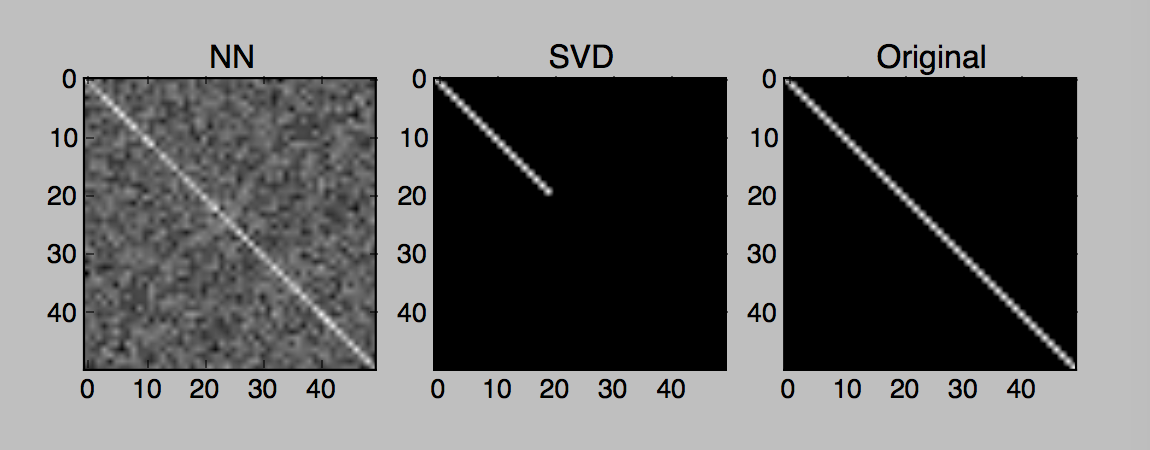
\includegraphics[width=0.45\textwidth,height=0.25\textheight,keepaspectratio]{identity_try_1}
\caption{NN, SVD, and Original versions of 50 $\times$ 50 identity matrix with rank 20 approximation.}
\label{fig:identity_try_1}
\end{figure}

\begin{figure}[H]
\centering
\begin{tabular}{|c|c|}
    \hline
    SVD Error (2-norm) & 1.0\\
    \hline
    NN Error (2-norm) & 1.00146298773\\
    \hline
    Error Difference & 0.00146\\
    \hline
\end{tabular}
\caption{Errors for matrix described in Figure~\ref{fig:identity_try_1}.}
\label{fig:identity_try_1_errors}
\end{figure}

\indent It is clear that the neural network did not pick up on the most important part of the rank 20 approximation, i.e. the first 20 singular values of the matrix. Interestingly the difference between the error for the SVD and NN approximations was 0.00146 where each error was around 1.0. That is incredibly low for such a difference visually.

\indent I then tried to approximate the matrix equal to the diagonal matrix that I call $M_n$ where each entry down the diagonal is equal to the row number that that entry is in. This matrix looks like $$M_n = \begin{pmatrix}1&0&\cdots&0\\0&2&\cdots&0\\\vdots&\vdots&\ddots&\vdots\\0&0&\cdots&n\end{pmatrix}$$ and the results of the neural net's approximation are shown in Figures~\ref{fig:identity_try_2}~\&~\ref{fig:identity_try_2_errors}.

\begin{figure}[H]
\centering
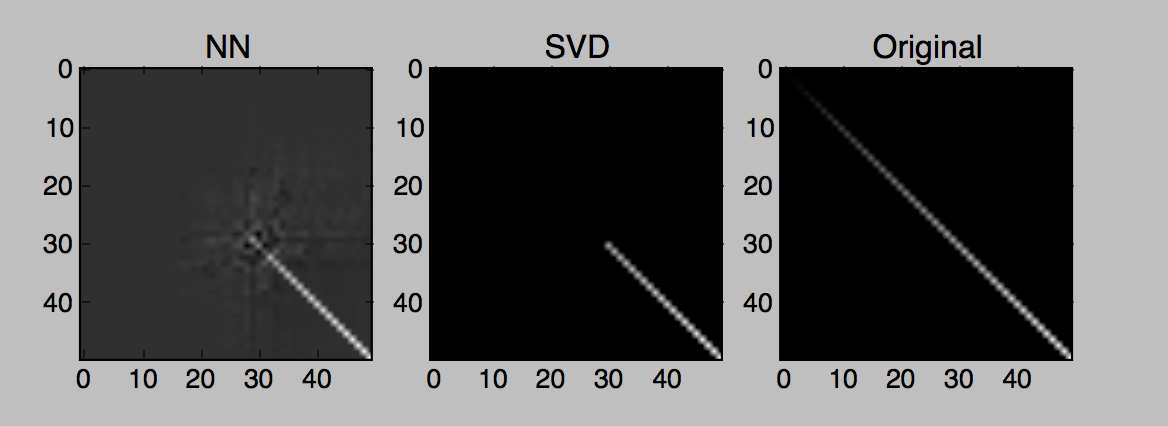
\includegraphics[width=0.45\textwidth,height=0.25\textheight,keepaspectratio]{identity_try_2}
\caption{NN, SVD, and Original versions of 50 $\times$ 50 $M_n$ matrix with rank 20 approximation.}
\label{fig:identity_try_2}
\end{figure}

\begin{figure}[H]
\centering
\begin{tabular}{|c|c|}
    \hline
    SVD Error (2-norm) & 0.591836734694\\
    \hline
    NN Error (2-norm) & 0.641697317379\\
    \hline
    Error Difference & 0.0499\\
    \hline
\end{tabular}
\caption{Errors for matrix described in Figure~\ref{fig:identity_try_2}.}
\label{fig:identity_try_2_errors}
\end{figure}

\indent This shows that the neural net is very good at approximating this matrix, at least visually. Even more interesting, however, is that the difference in the errors is actually higher than it was with just the identity matrix. This test yielded an error of 0.5918 for the SVD approximation, and an error of 0.6417 for the neural net approximation which gives a difference of 0.0499. This is somewhat expected, however, because this is a more complex matrix than the identity.

\subsection{Approximating Random Low Dimension Matrices}
\noindent Through our tests, the neural net gave the most variation in results when we ran it on low rank approximations of low dimension matrices. The tests enumerated in this section focus on matrices of size $n=10$ or smaller.


%In practice, and given the limitations of time and processing power, the neural net rarely performs optimally. 
%\includegraphics[width=0.44\textwidth,height=\textheight,keepaspectratio]{identity-10}

%restructure - should define & explain all the math before getting into implementation and results
%briefly define rank
%explain epoch in neural net section

\end{document}
